\newpage

\begin{figure}
    \centering
    \begin{subfigure}{0.5\textwidth}
    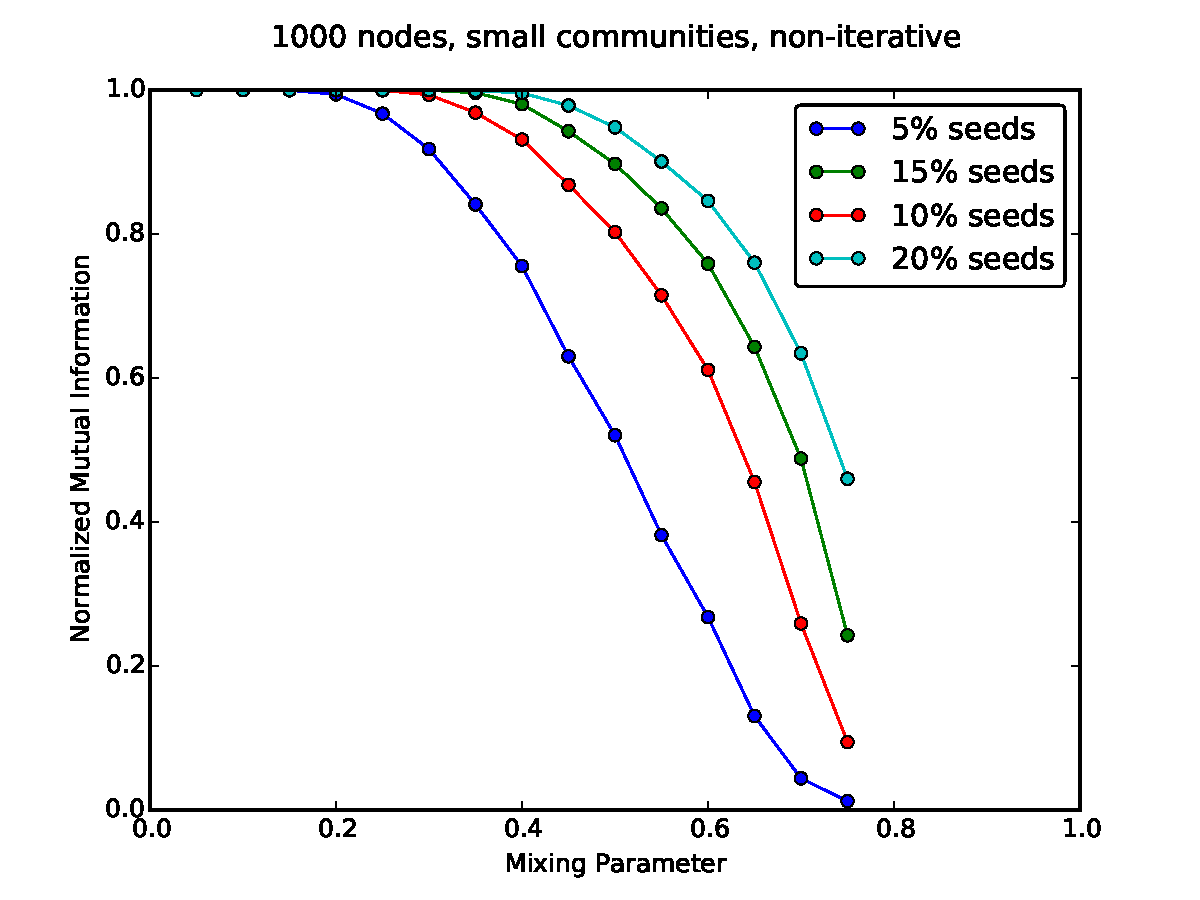
\includegraphics[width=\linewidth]{plots/nonoverlap_noniter_a.pdf}
    \end{subfigure}%
    \begin{subfigure}{0.5\textwidth}
    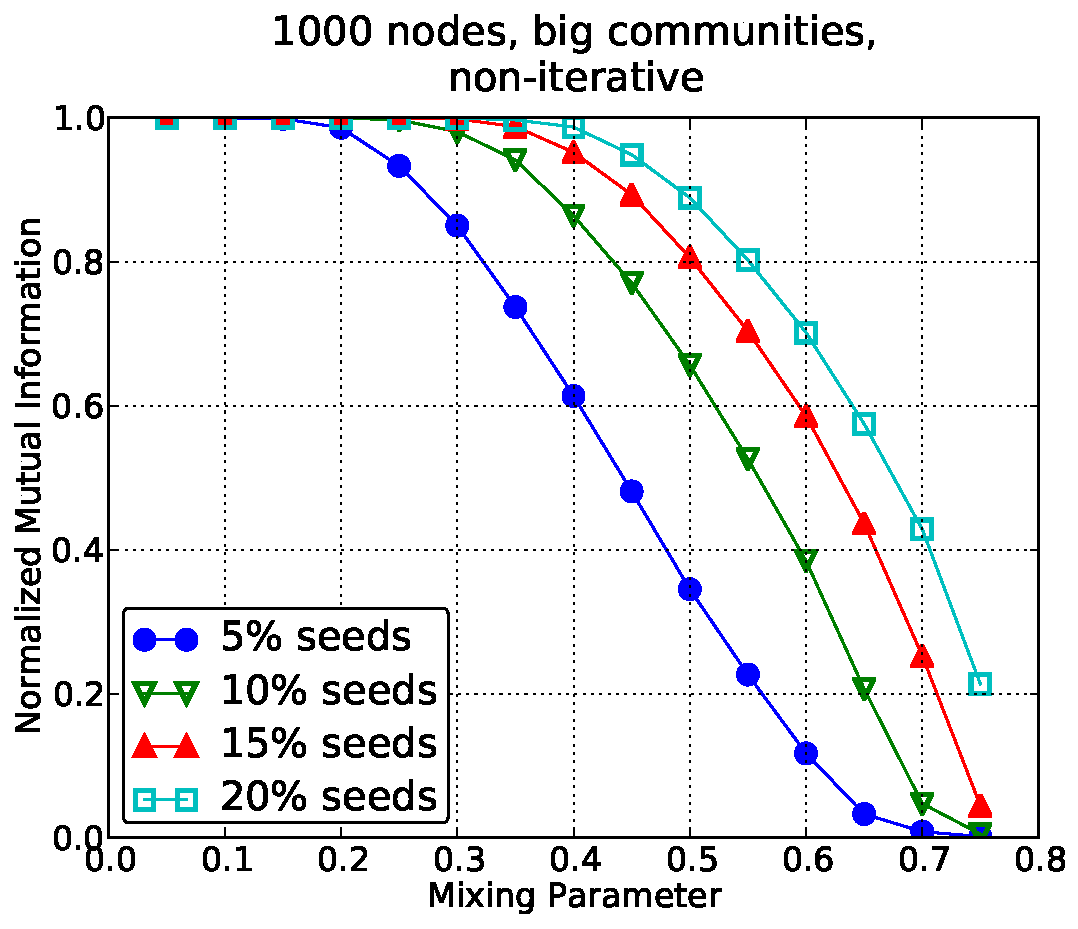
\includegraphics[width=\linewidth]{plots/nonoverlap_noniter_b.pdf}
    \end{subfigure}
    \begin{subfigure}{0.5\textwidth}
    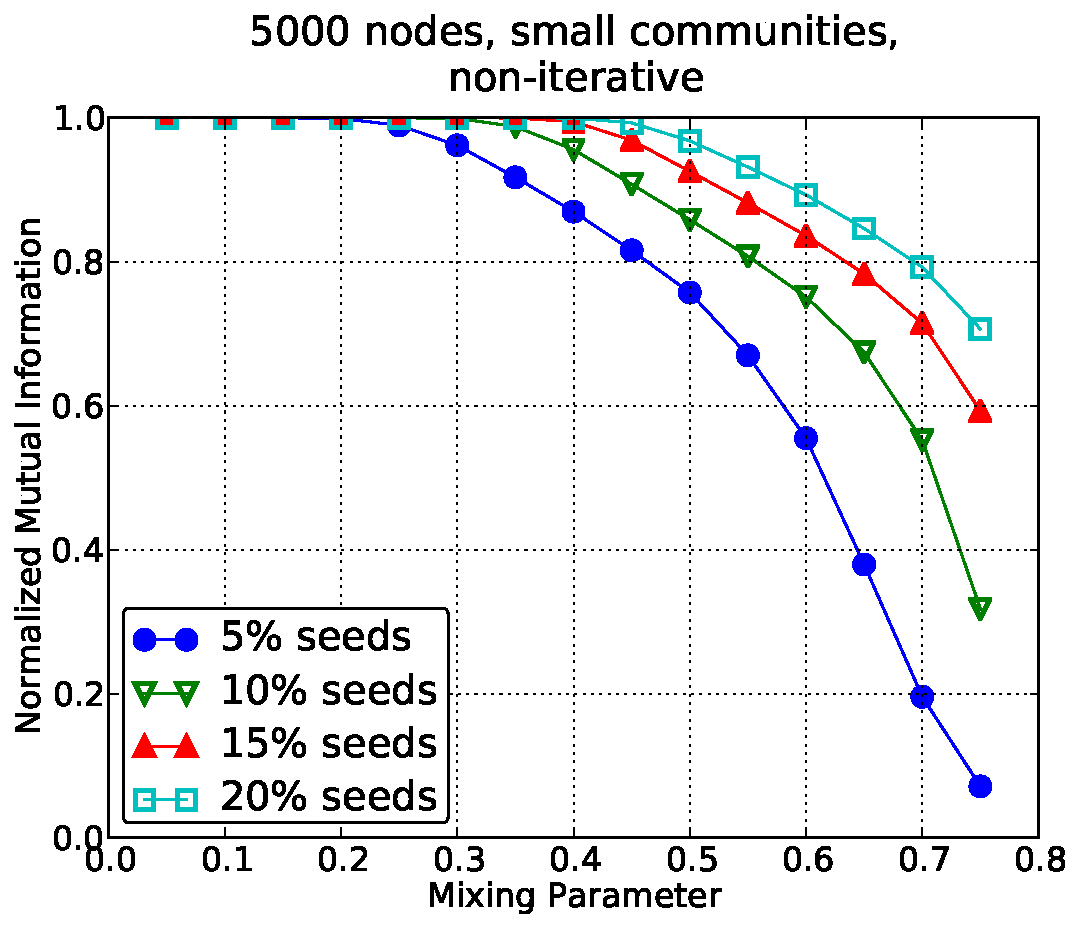
\includegraphics[width=\linewidth]{plots/nonoverlap_noniter_c.pdf}
    \end{subfigure}%
    \begin{subfigure}{0.5\textwidth}
    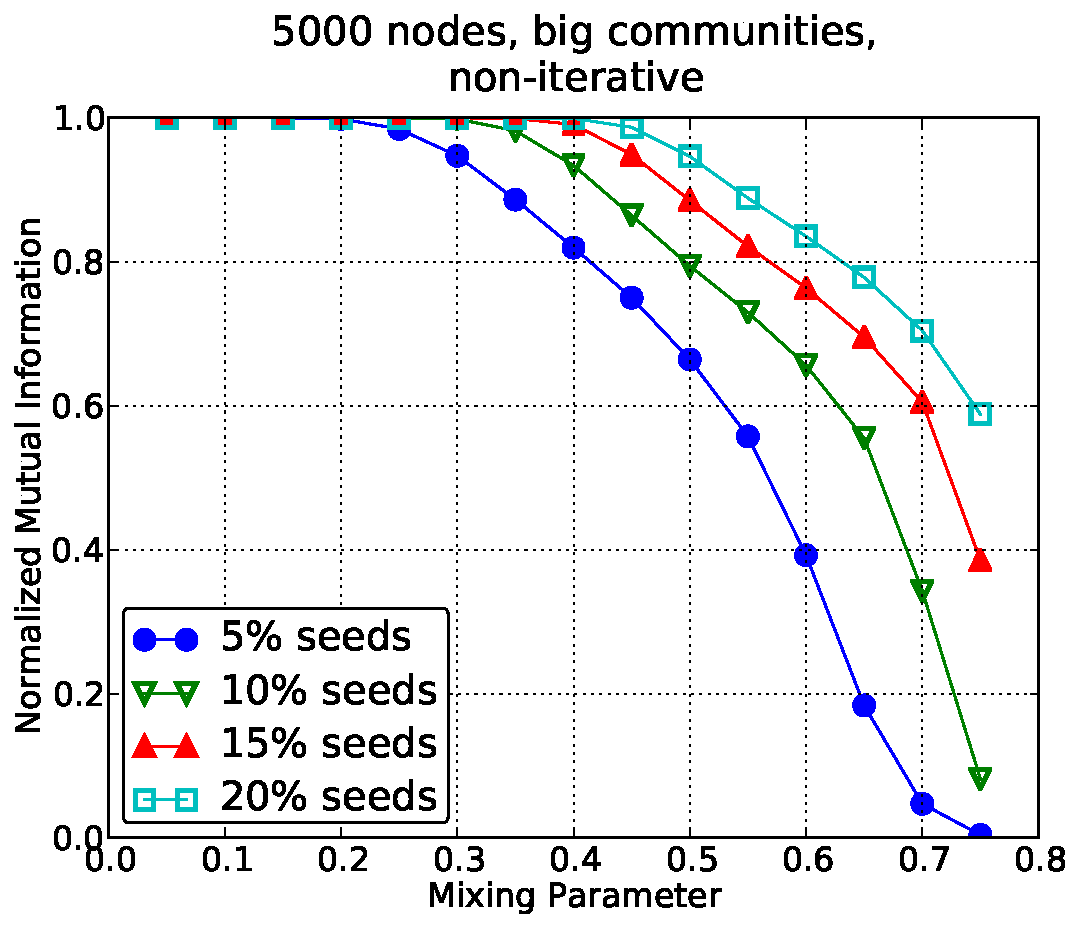
\includegraphics[width=\linewidth]{plots/nonoverlap_noniter_d.pdf}
    \end{subfigure}
    \caption{Noniterative method for nonoverlapping communities.}
\end{figure}

\begin{figure}
    \centering
    \begin{subfigure}{0.5\textwidth}
    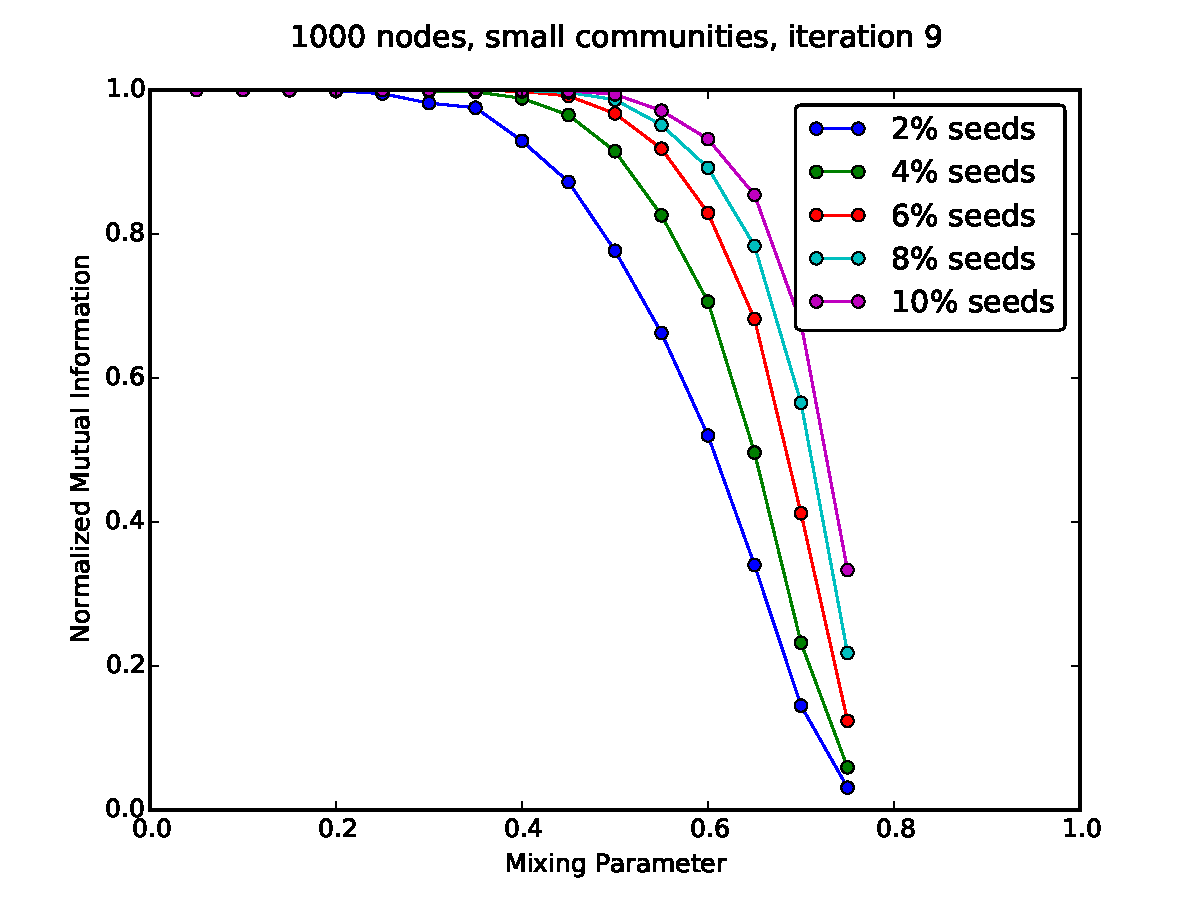
\includegraphics[width=\linewidth]{plots/nonoverlap_iter_a.pdf}
    \end{subfigure}%
    \begin{subfigure}{0.5\textwidth}
    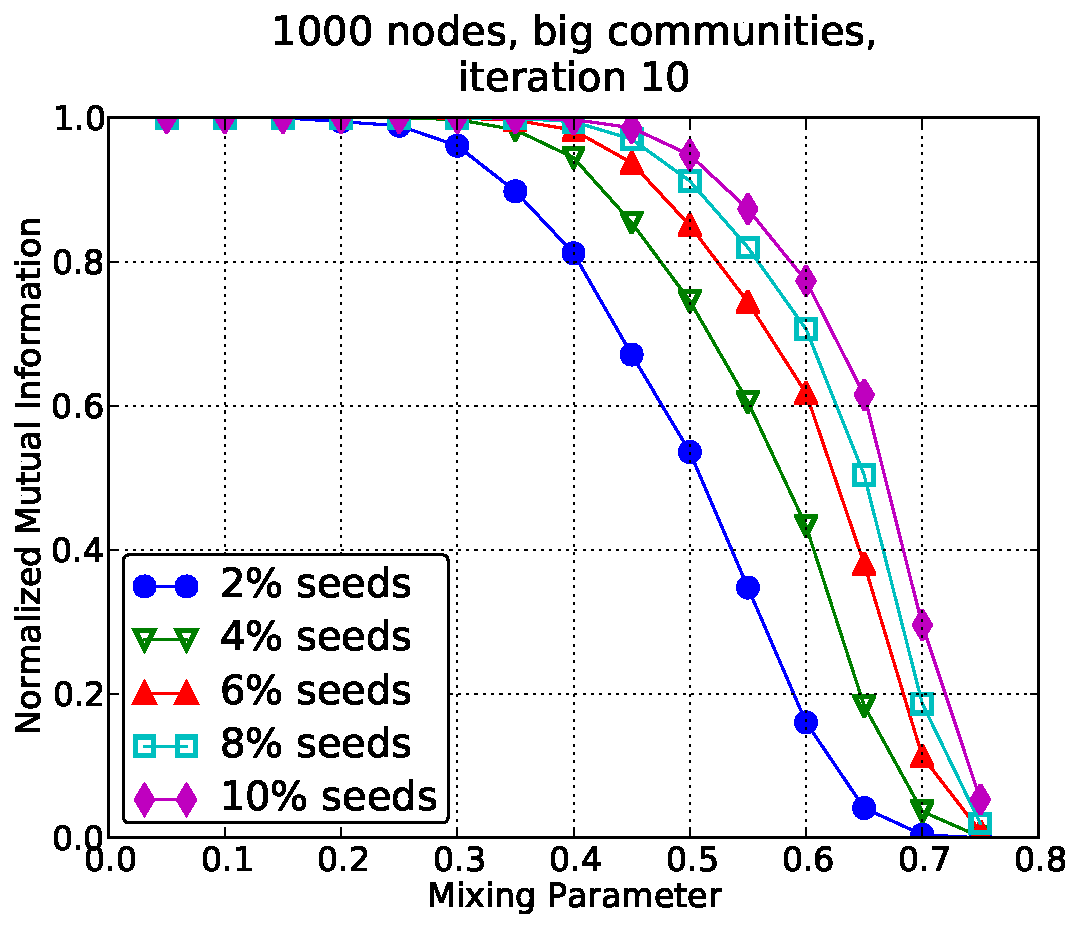
\includegraphics[width=\linewidth]{plots/nonoverlap_iter_b.pdf}
    \end{subfigure}
    \begin{subfigure}{0.5\textwidth}
    %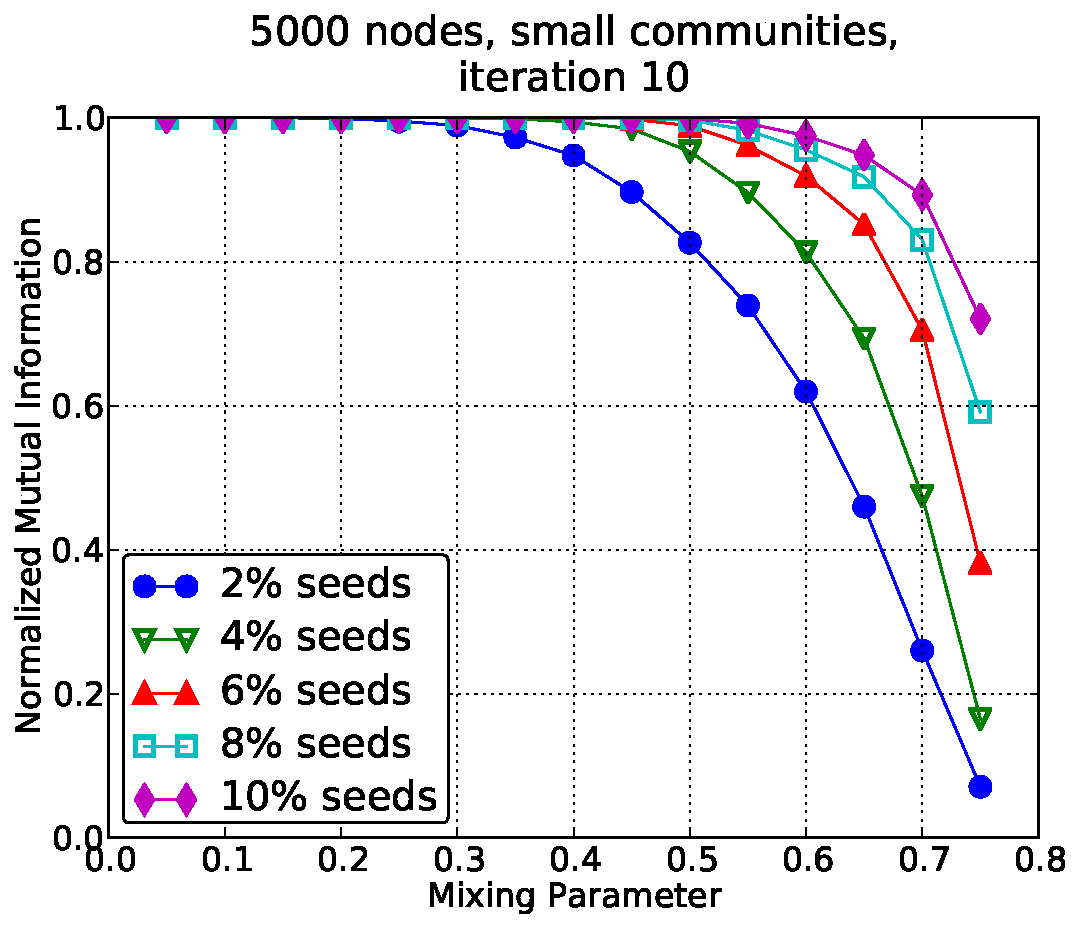
\includegraphics[width=\linewidth]{plots/nonoverlap_iter_c.pdf}
    
\includegraphics[width=\linewidth]{plots/placeholder.pdf}
    \end{subfigure}%
    \begin{subfigure}{0.5\textwidth}
    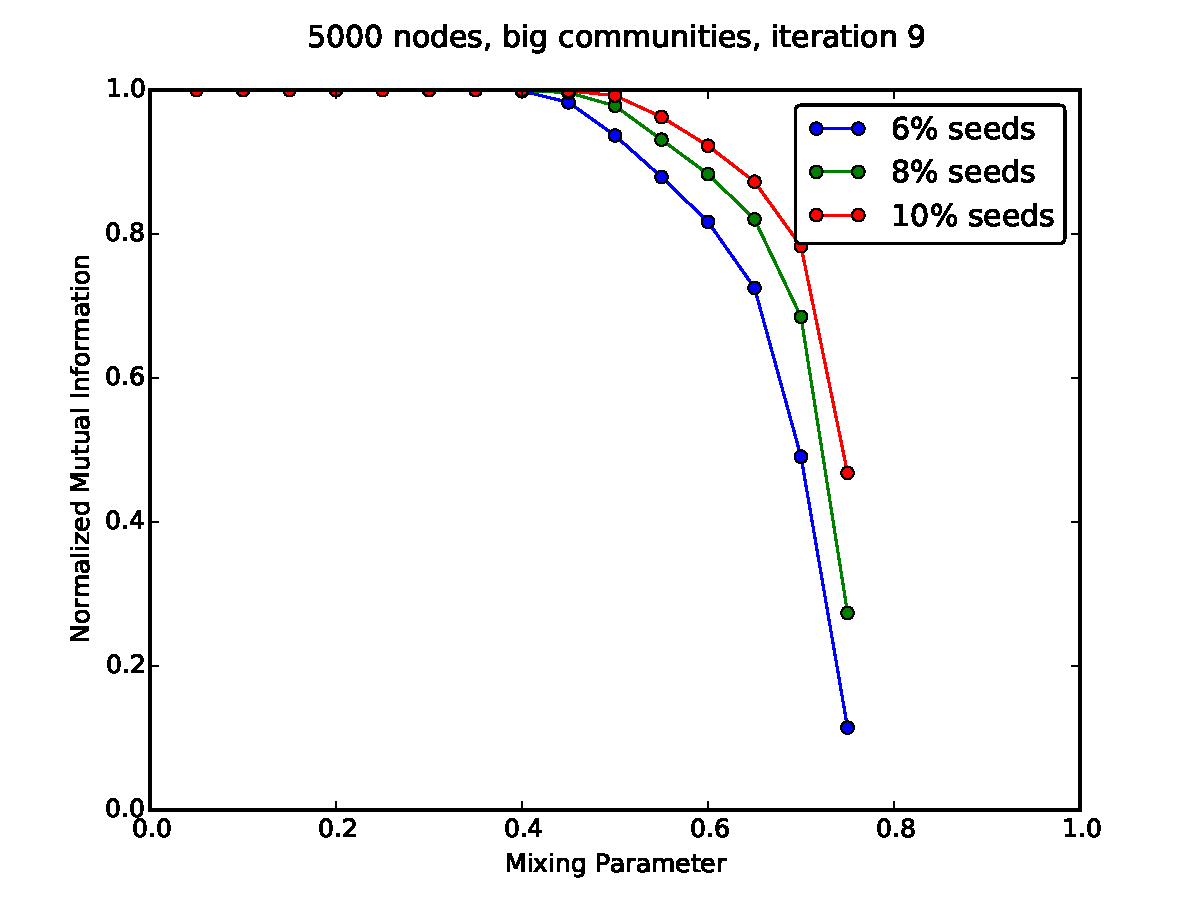
\includegraphics[width=\linewidth]{plots/nonoverlap_iter_d.pdf}
    \end{subfigure}
    \caption{Iterative method for nonoverlapping communities.}
\end{figure}

\begin{figure}
    \centering
    \begin{subfigure}{0.5\textwidth}
    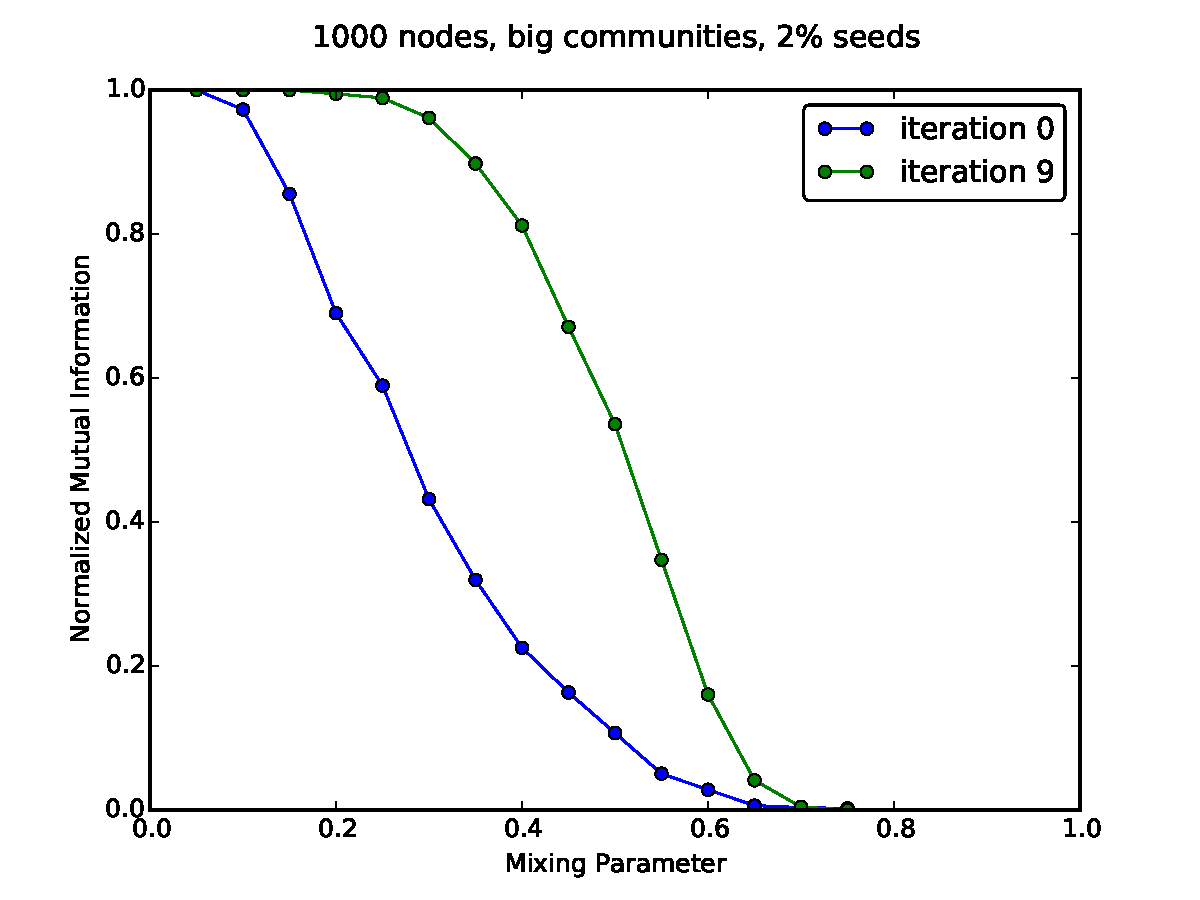
\includegraphics[width=\linewidth]{plots/nonoverlap_compare_a.pdf}
    \end{subfigure}%
    \begin{subfigure}{0.5\textwidth}
    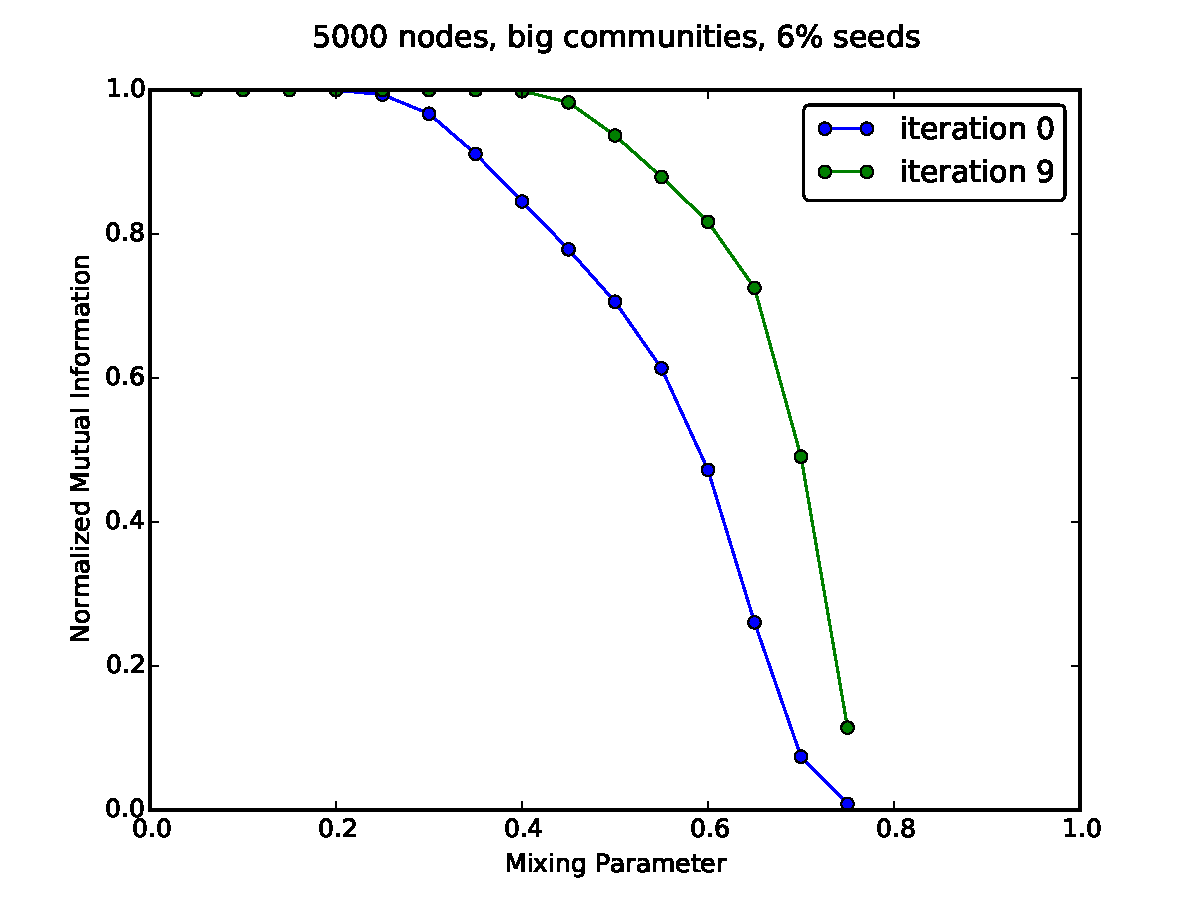
\includegraphics[width=\linewidth]{plots/nonoverlap_compare_b.pdf}
    \end{subfigure}
    \caption{Comparison between the the iterative and non-iterative method for non-overlapping communities.}
\end{figure}


\begin{figure}
    \centering
    \begin{subfigure}{0.5\textwidth}
    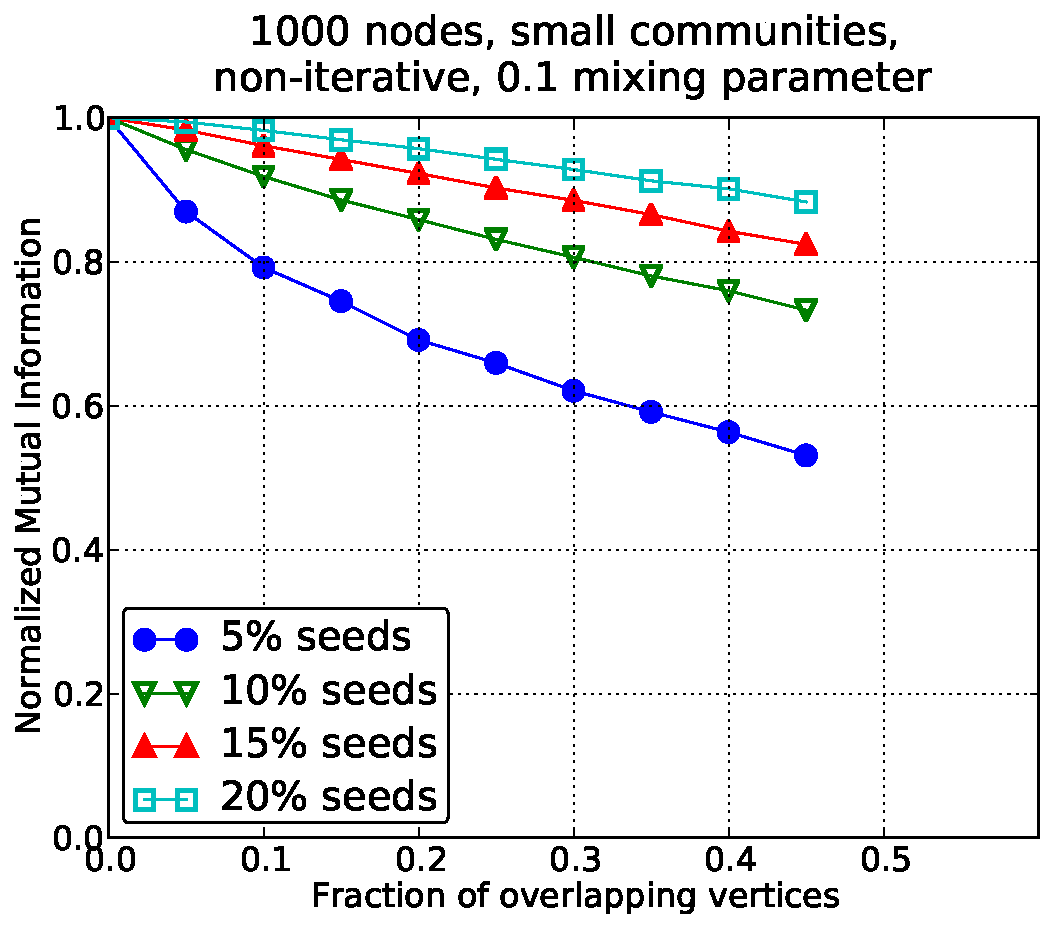
\includegraphics[width=\linewidth]{plots/overlap_noniter_1mu_a.pdf}
    \end{subfigure}%
    \begin{subfigure}{0.5\textwidth}
    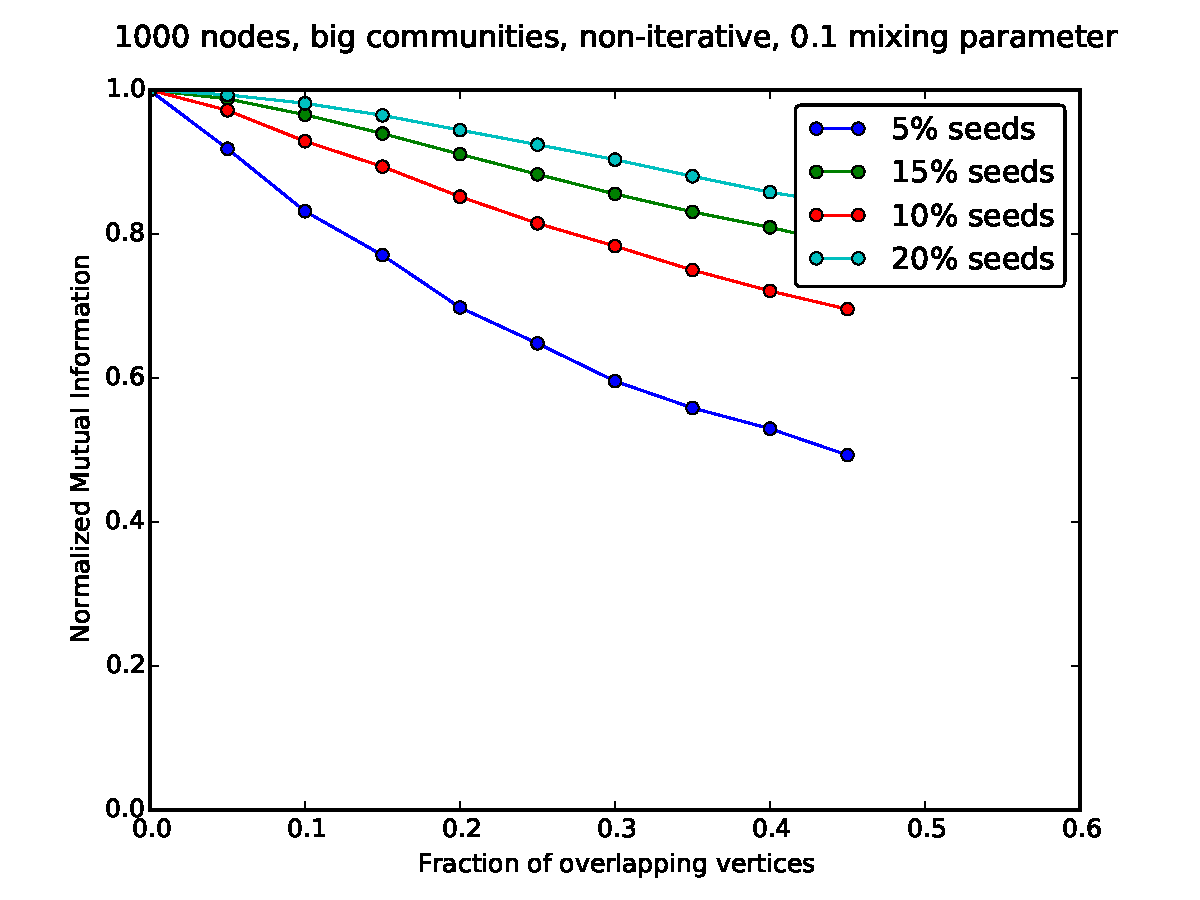
\includegraphics[width=\linewidth]{plots/overlap_noniter_1mu_b.pdf}
    \end{subfigure}
    \begin{subfigure}{0.5\textwidth}
    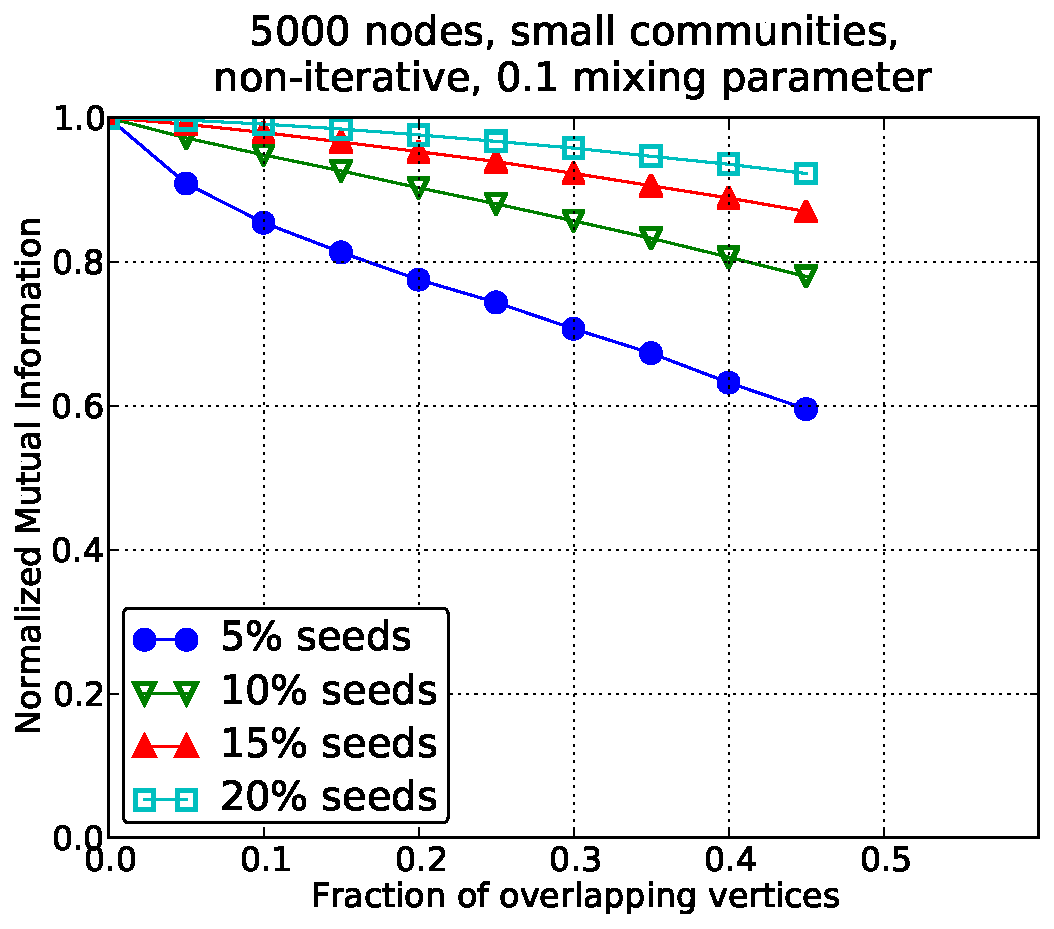
\includegraphics[width=\linewidth]{plots/overlap_noniter_1mu_c.pdf}
    \end{subfigure}%
    \begin{subfigure}{0.5\textwidth}
    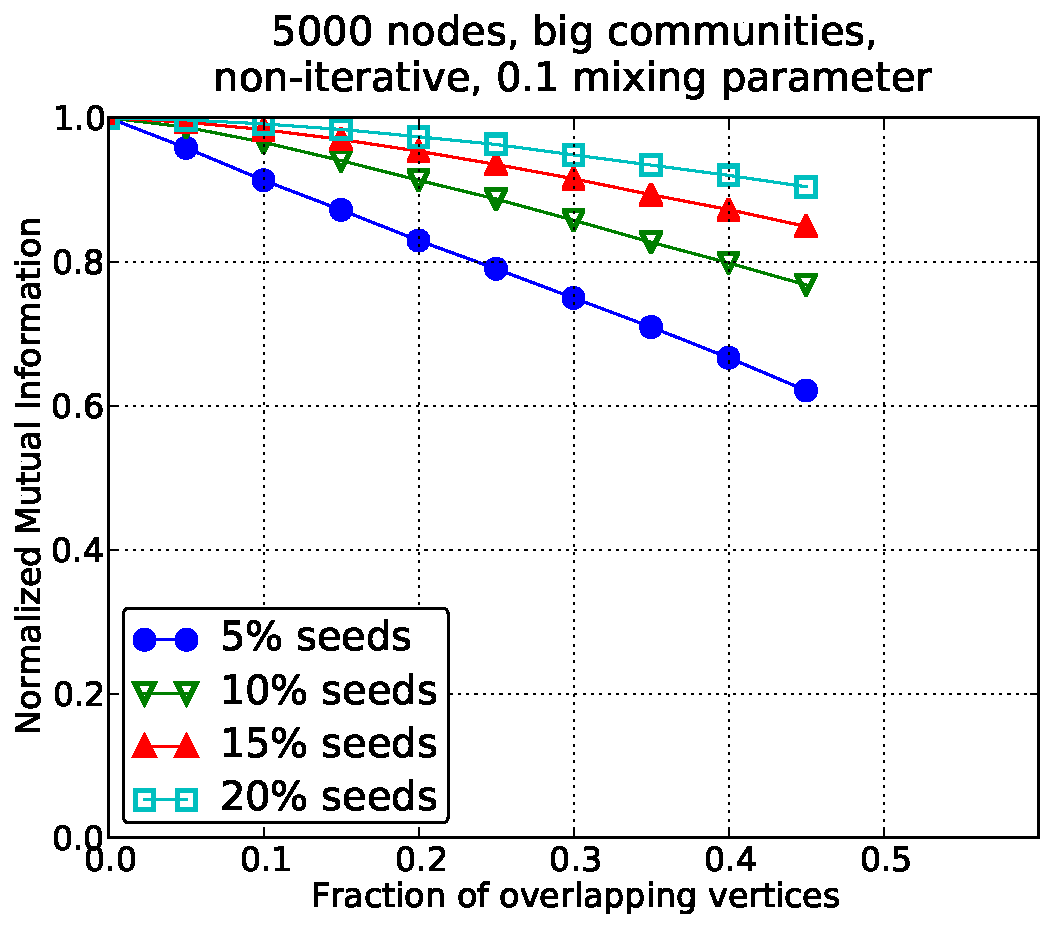
\includegraphics[width=\linewidth]{plots/overlap_noniter_1mu_d.pdf}
    \end{subfigure}
    \begin{subfigure}{0.5\textwidth}
    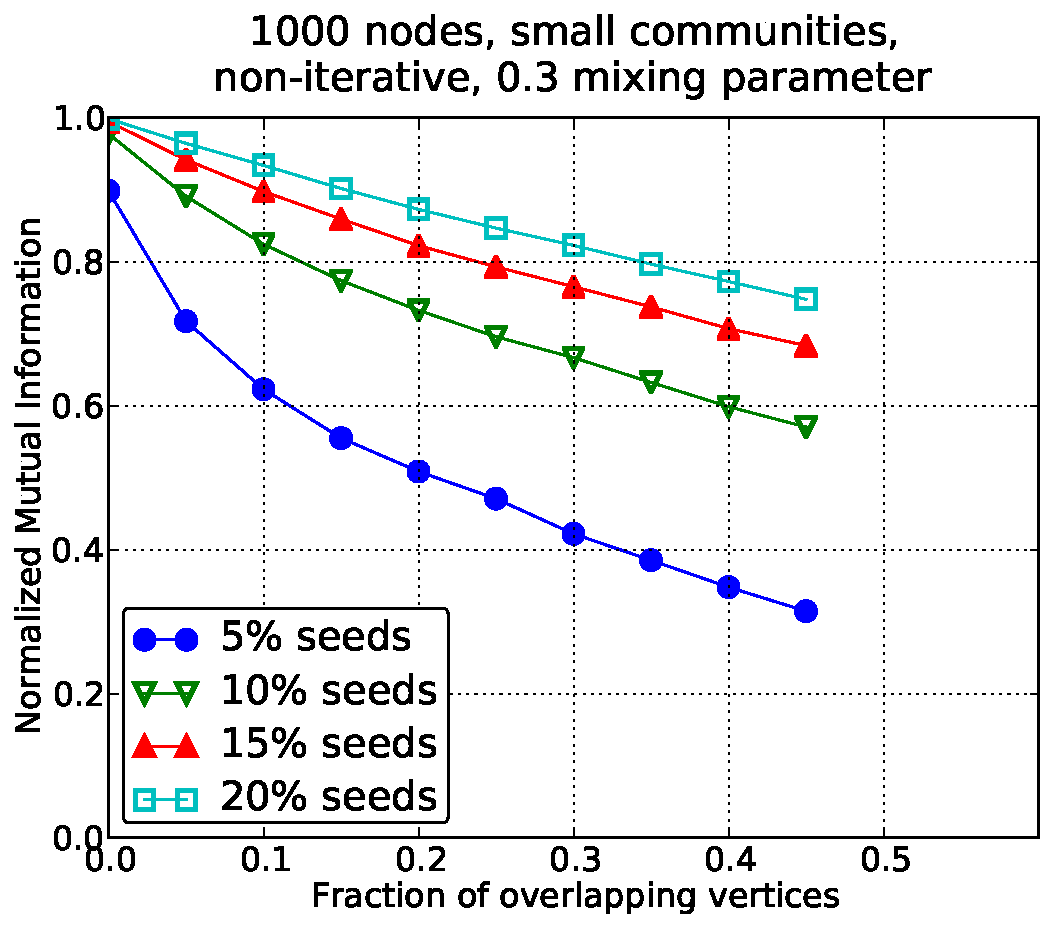
\includegraphics[width=\linewidth]{plots/overlap_noniter_3mu_a.pdf}
    \end{subfigure}%
    \begin{subfigure}{0.5\textwidth}
    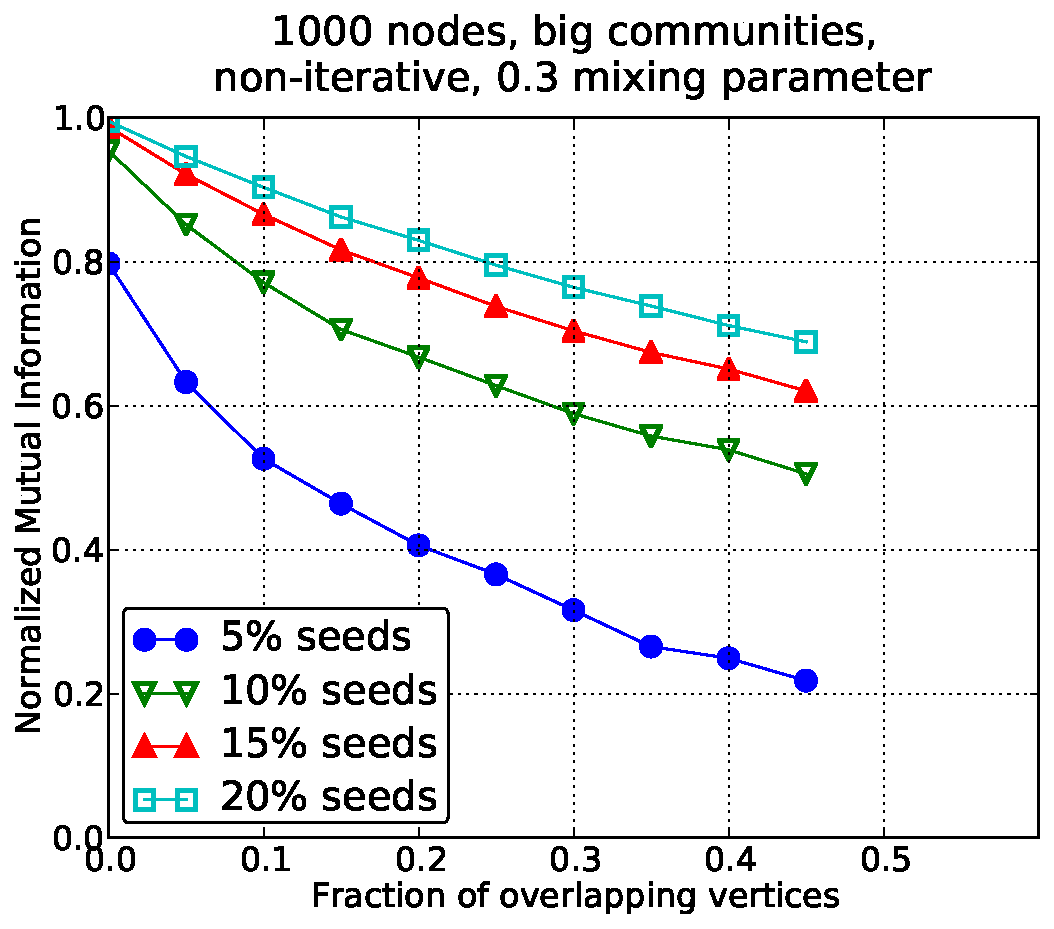
\includegraphics[width=\linewidth]{plots/overlap_noniter_3mu_b.pdf}
    \end{subfigure}
    \begin{subfigure}{0.5\textwidth}
    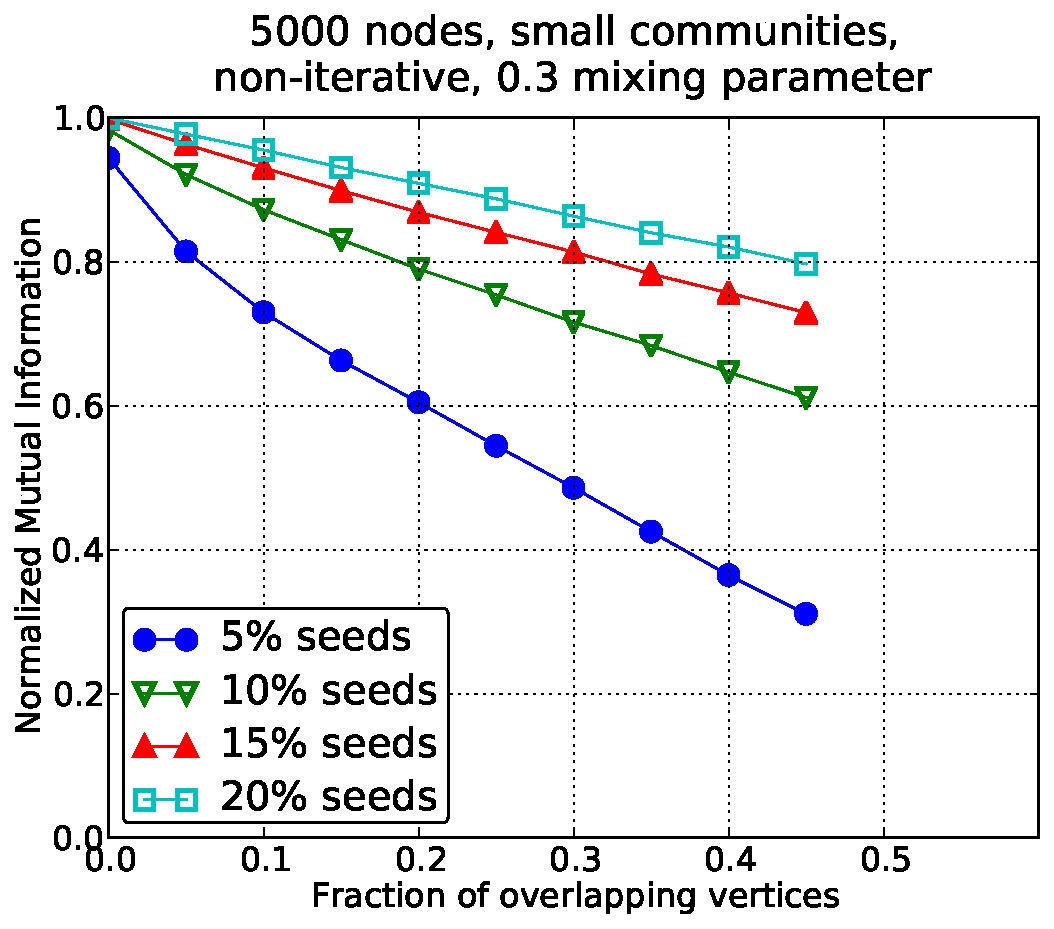
\includegraphics[width=\linewidth]{plots/overlap_noniter_3mu_c.pdf}
    \end{subfigure}%
    \begin{subfigure}{0.5\textwidth}
    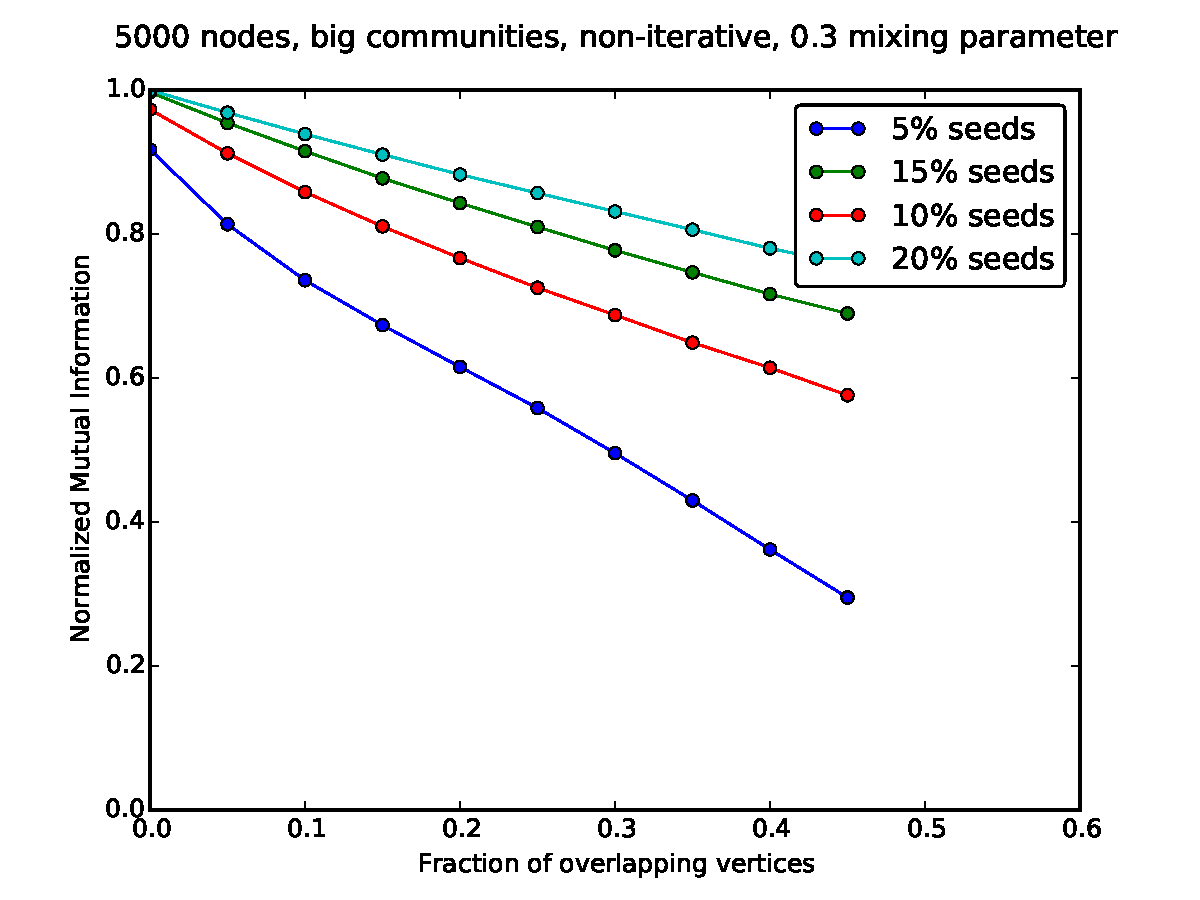
\includegraphics[width=\linewidth]{plots/overlap_noniter_3mu_d.pdf}
    \end{subfigure}
    \caption{Noniterative method for overlapping communities.}
\end{figure}


\begin{figure}
    \centering
    \begin{subfigure}{0.5\textwidth}
    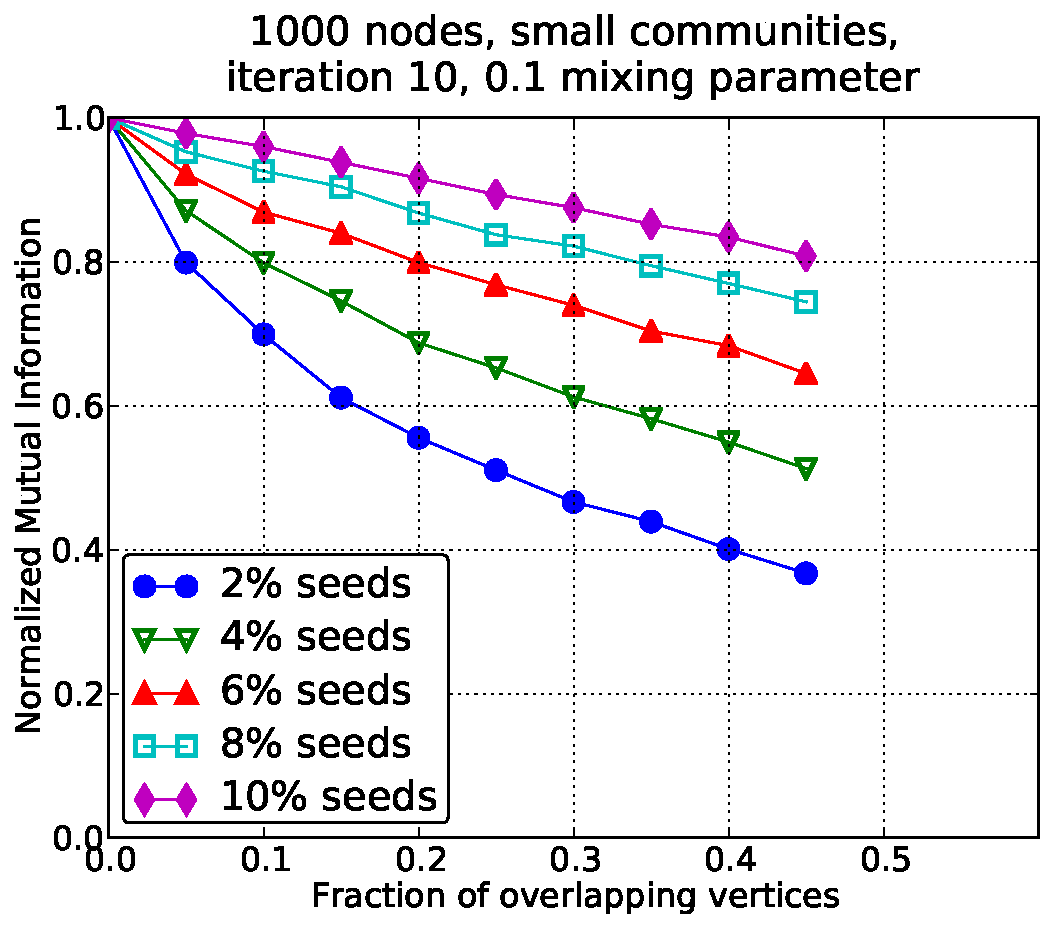
\includegraphics[width=\linewidth]{plots/overlap_iter_1mu_a.pdf}
    \end{subfigure}%
    \begin{subfigure}{0.5\textwidth}
    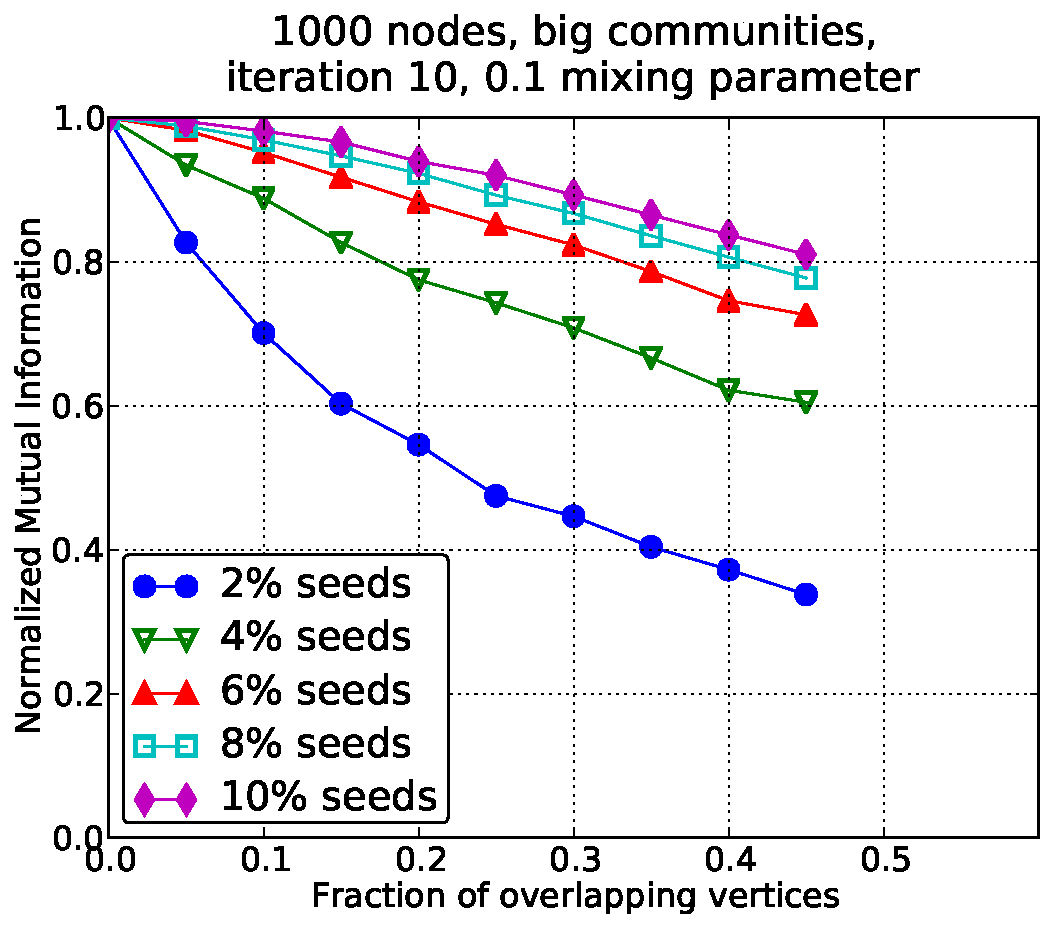
\includegraphics[width=\linewidth]{plots/overlap_iter_1mu_b.pdf}
    \end{subfigure}
    \begin{subfigure}{0.5\textwidth}
    
\includegraphics[width=\linewidth]{plots/placeholder.pdf}
    %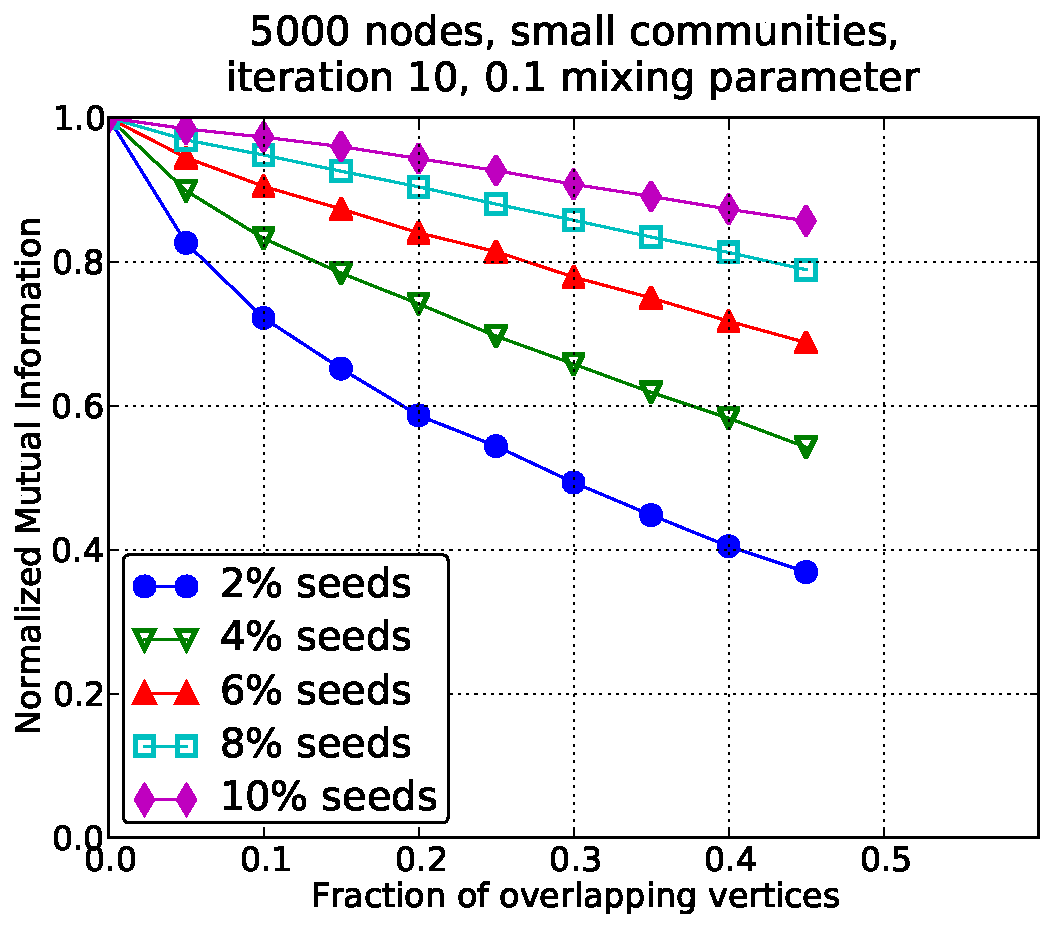
\includegraphics[width=\linewidth]{plots/overlap_iter_1mu_c.pdf}
    \end{subfigure}%
    \begin{subfigure}{0.5\textwidth}
    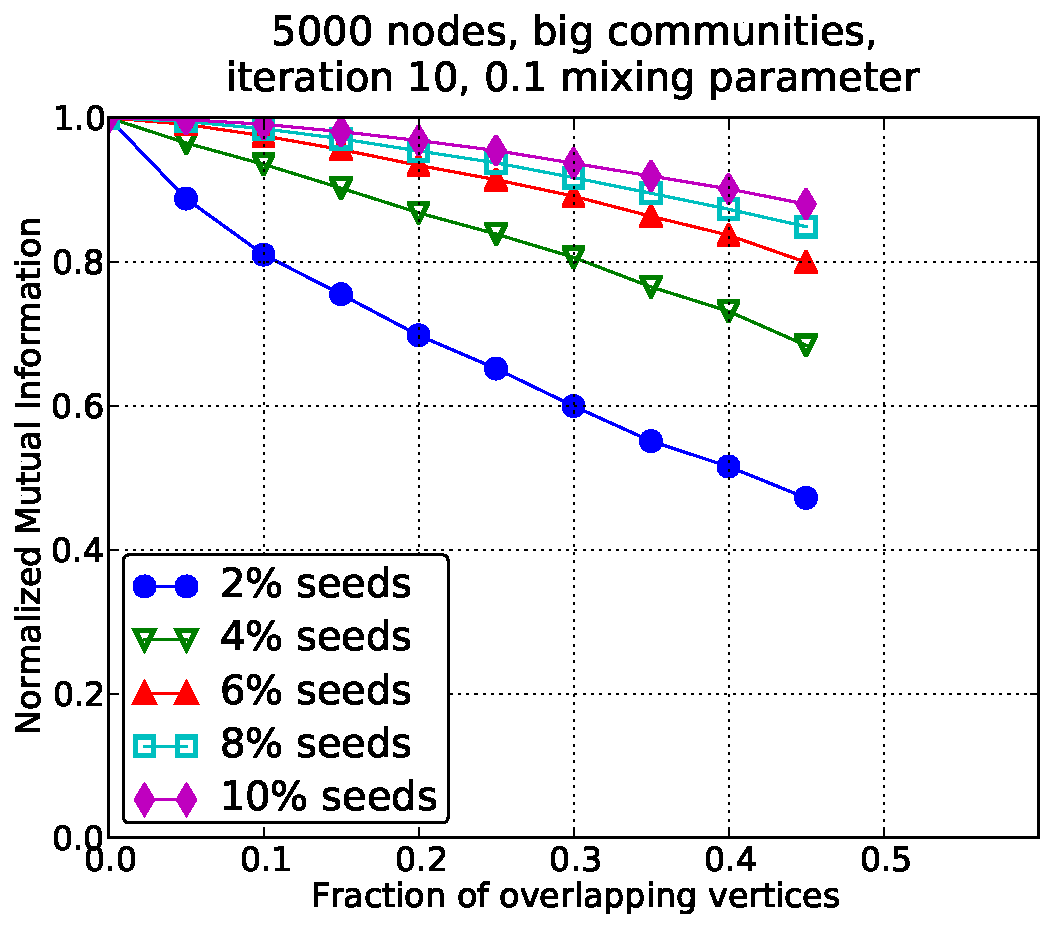
\includegraphics[width=\linewidth]{plots/overlap_iter_1mu_d.pdf}
    \end{subfigure}
    \begin{subfigure}{0.5\textwidth}
    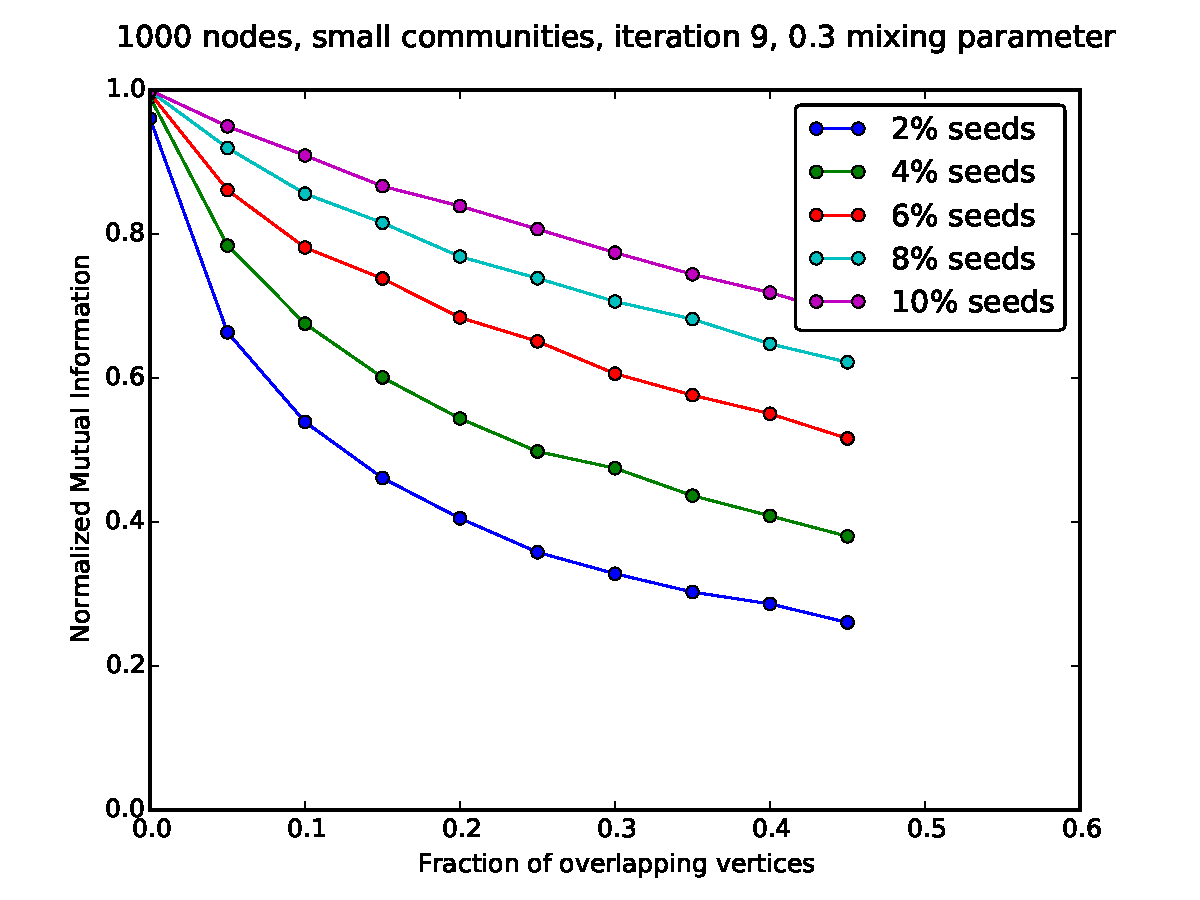
\includegraphics[width=\linewidth]{plots/overlap_iter_3mu_a.pdf}
    \end{subfigure}%
    \begin{subfigure}{0.5\textwidth}
    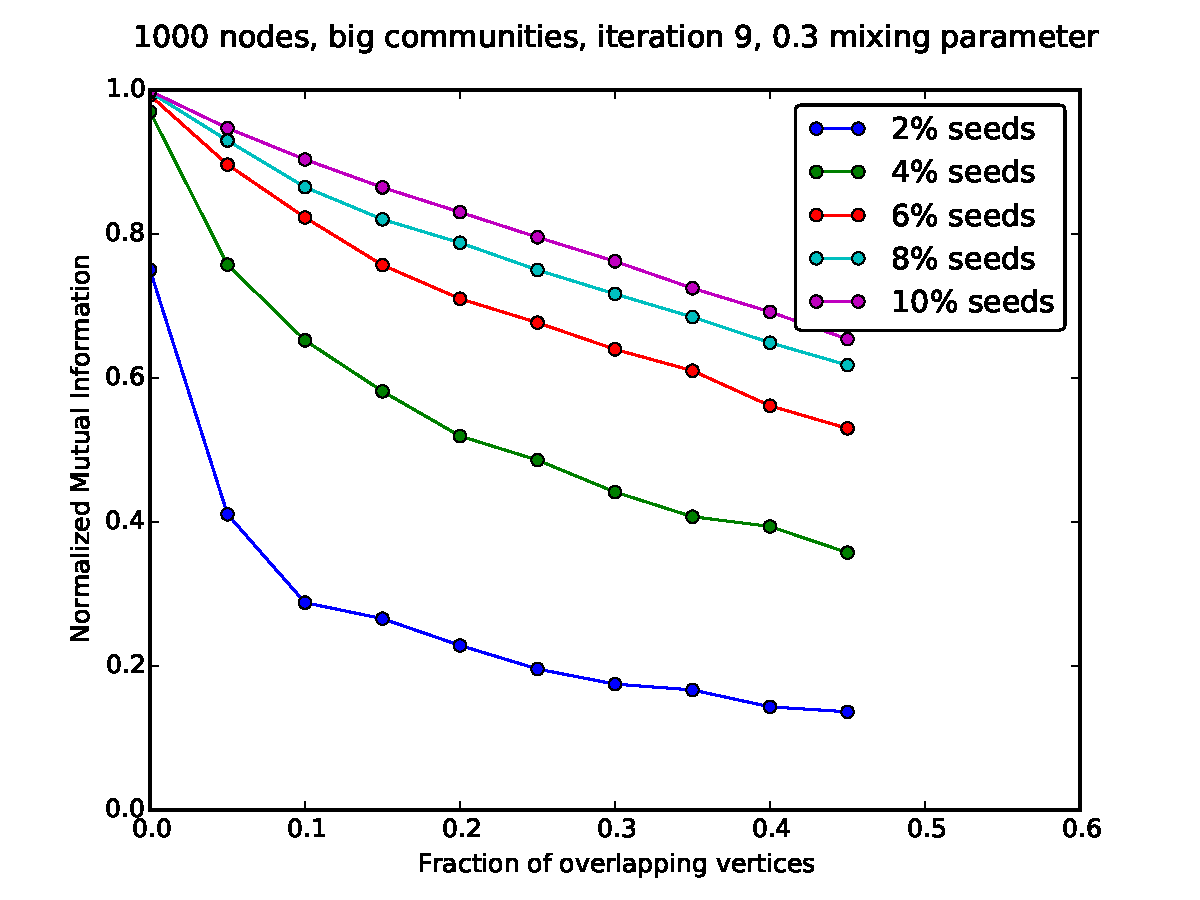
\includegraphics[width=\linewidth]{plots/overlap_iter_3mu_b.pdf}
    \end{subfigure}
    \begin{subfigure}{0.5\textwidth}
    
\includegraphics[width=\linewidth]{plots/placeholder.pdf}
    %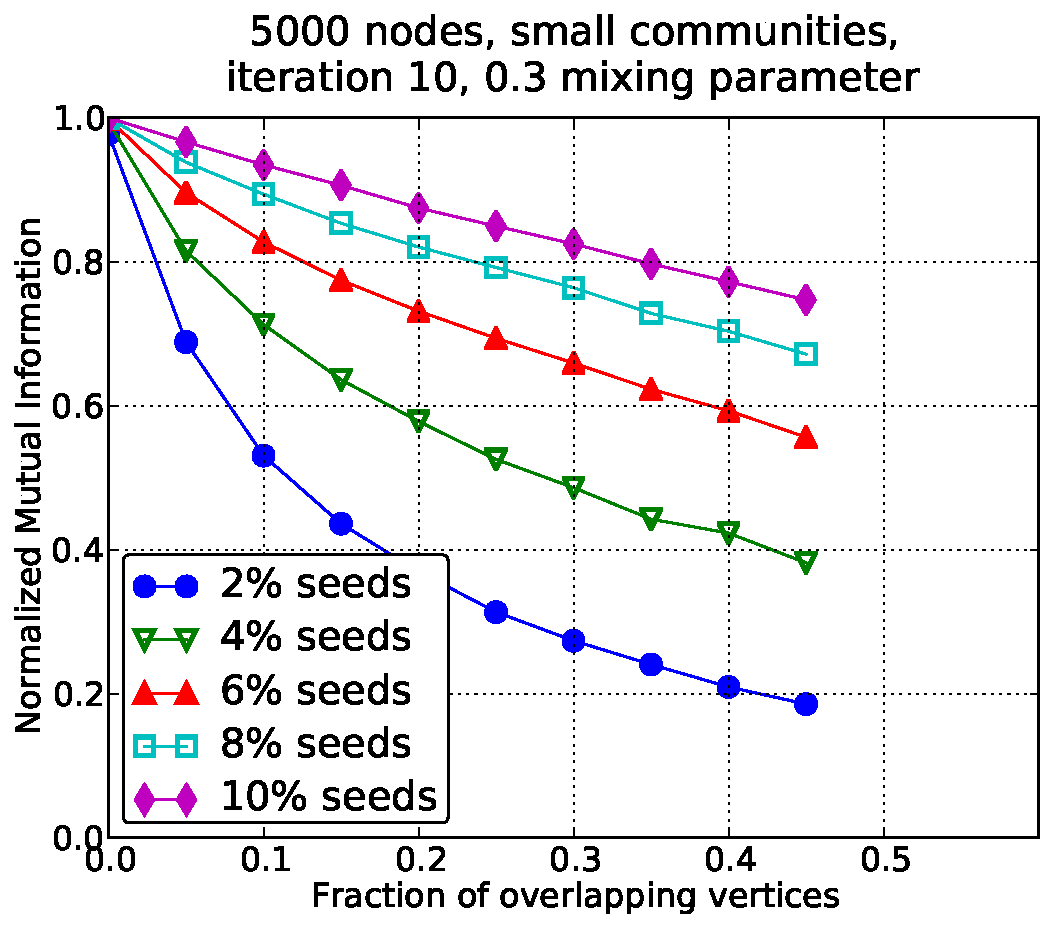
\includegraphics[width=\linewidth]{plots/overlap_iter_3mu_c.pdf}
    \end{subfigure}%
    \begin{subfigure}{0.5\textwidth}
    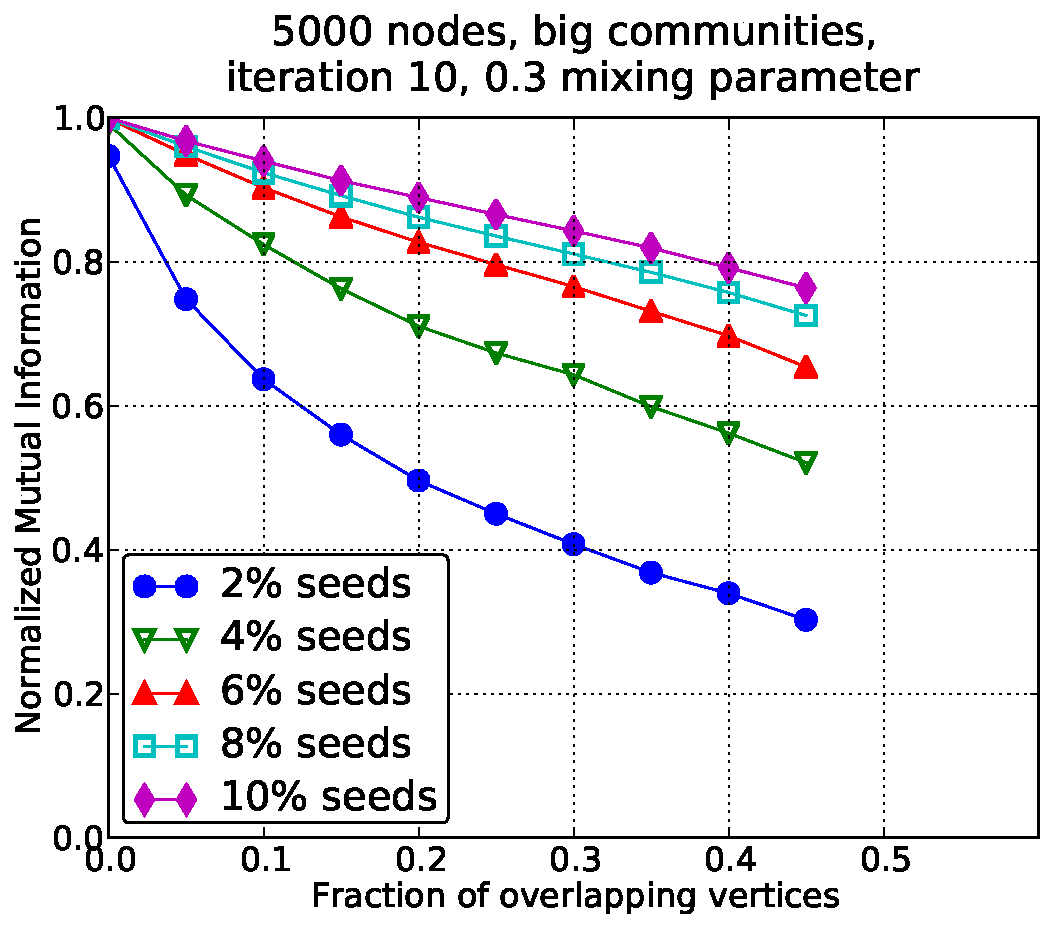
\includegraphics[width=\linewidth]{plots/overlap_iter_3mu_d.pdf}
    \end{subfigure}
    \caption{Iterative method for overlapping communities.}
\end{figure}

\begin{figure}
    \centering
    \begin{subfigure}{0.5\textwidth}
    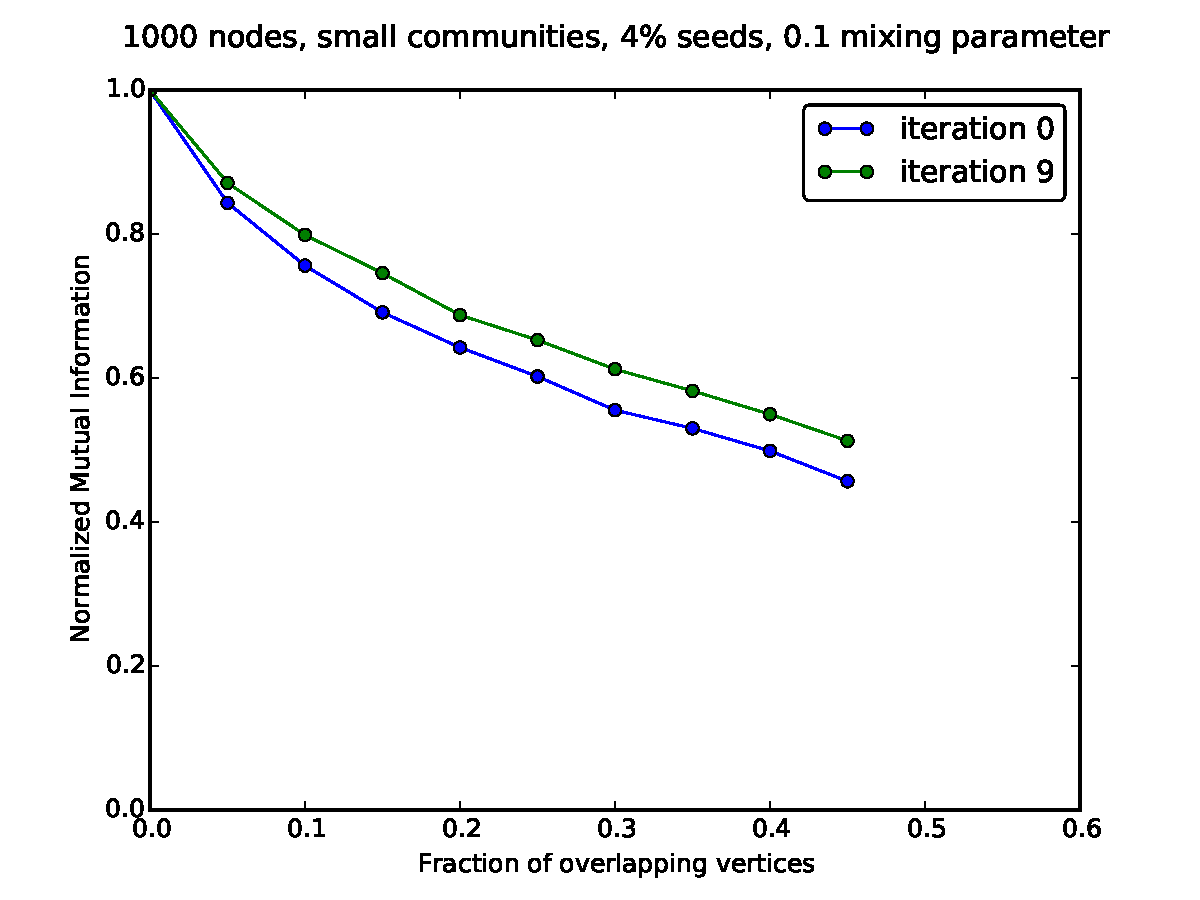
\includegraphics[width=\linewidth]{plots/overlap_compare_a.pdf}
    \end{subfigure}%
    \begin{subfigure}{0.5\textwidth}
    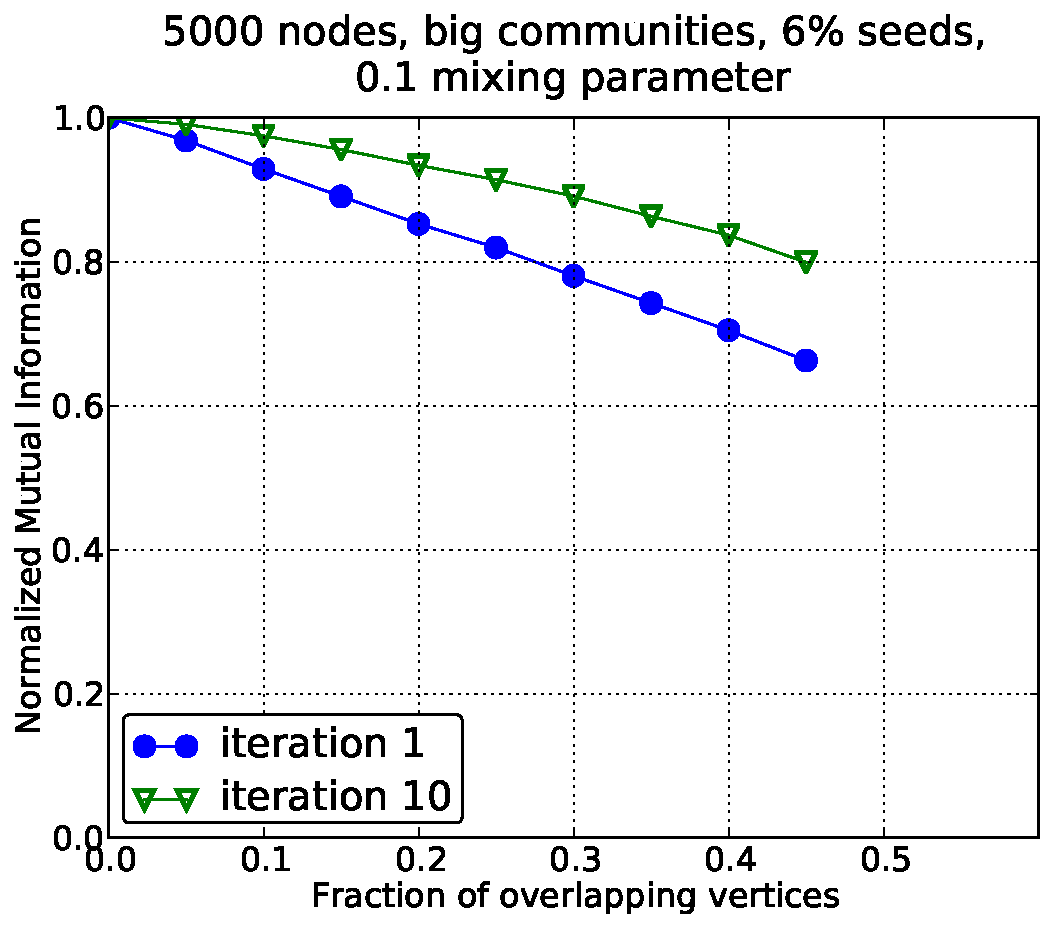
\includegraphics[width=\linewidth]{plots/overlap_compare_b.pdf}
    \end{subfigure}
    \caption{Comparison between the the iterative and non-iterative method for overlapping communities.}
\end{figure}


